% !TeX program = pdflatex
% Categorical Structure Transfer in Belief Networks
% Target venue: NeurIPS 2026 Workshop (ML4PS / Probabilistic Programming)
% or UAI / AISTATS short track. Main-track submission would require a
% non-curated benchmark suite (§Limitations #1).

\documentclass{article}
\usepackage[utf8]{inputenc}
\usepackage[T1]{fontenc}
\usepackage{microtype}
\usepackage[margin=1in]{geometry}
\usepackage{graphicx}
\usepackage{booktabs}
\usepackage{amsmath,amssymb,amsthm}
\newtheorem{proposition}{Proposition}
\newtheorem{definition}{Definition}
\newtheorem{claim}{Claim}
\usepackage{url}
\usepackage{hyperref}
\usepackage{xcolor}
\usepackage{caption}
\usepackage{subcaption}
\usepackage{algorithm}
\usepackage{algpseudocode}
\usepackage{natbib}
\usepackage{enumitem}

\hypersetup{
  colorlinks=true,
  linkcolor=blue!50!black,
  citecolor=blue!50!black,
  urlcolor=blue!60!black
}

\title{\textbf{Categorical Structure Transfer in Belief Networks}}

\author{%
  Anonymous submission\\
}

\date{}

\begin{document}

\maketitle

\begin{abstract}
\noindent
Two physical-reasoning problems --- ``voltage decays in an RC circuit''
and ``concentration decays in a first-order chemical reaction'' --- share
the same functional form $y(t) = y_{0} \cdot e^{-k t}$ despite operating
in different domains at different numerical scales. A probabilistic
reasoning system should be able to recognise this equivalence and
transfer class-level knowledge from one domain to another.

We present an end-to-end pipeline that (i)~represents each belief
network via four equivalent signature layers — op-multiset, Weisfeiler-
Lehman, symbolic Markov-category shape, Blackwell-Sherman-Stein
likelihood equality — all four of which recover the
$3$-class law-zoo partition by construction, since the law-zoo
fixtures were built with one canonical $\mu(\theta, t)$ function per
class; (ii)~retrieves equivalent networks via Ruzicka distance on the
op multiset; and (iii)~transfers posterior log-SDs (class-level
precision) from a data-rich source to a data-poor target, without
transferring any scale-specific information.

\textbf{The signature-stack agreement (ARI $= 1.00$) is therefore
largely by construction, not a discovered phenomenon. The
non-tautological empirical result is the transfer behaviour}: on
few-shot saturation-class targets, prior-SD transfer through the
signature gate delivers a mean $89.5\%$ held-out MSE reduction
against an uninformed cold-start; on exp\_decay-class targets it
delivers no improvement (a dynamical asymmetry stemming from how
decay vs plateau couples to parameter identifiability; we report
this rather than smooth it over). We also release a trained GNN
embedding that matches the symbolic clustering, but openly note that
a random-initialised MPNN matches it equally well on this fixture,
making the GNN's empirical contribution null; we position the GNN
as future-work infrastructure for a law-zoo v3 with within-class
graph variation and make this limitation precise rather than imply
a training effect.
\end{abstract}

\section{Introduction}
\label{sec:intro}

Classical Bayesian hierarchical models capture the intuition that
related tasks should share a hyperprior, but they require the
modeller to \emph{declare} the shared structure up front. Meta-learning
approaches \citep{finn2017maml} learn a good initialisation across
tasks but treat tasks as opaque. Neither approach addresses the
\emph{discovery} question: given two belief networks built independently,
can a system infer that they are instances of one underlying
abstraction?

This paper proposes an operational answer. Two belief networks
$\mathcal{B}_{a}$ and $\mathcal{B}_{b}$ are declared
\emph{structurally equivalent} iff they produce the same
\textbf{StructuralSignature} --- a canonical hash derived from the
PyTensor op graph rooted at their observed random variables. Equivalence
detected this way supports three downstream operations:

\begin{itemize}[leftmargin=*, itemsep=0pt]
\item \textbf{Retrieval:} nearest-neighbour lookup in a signature
  library, using a Ruzicka (weighted-Jaccard) distance on op multisets
  that agrees with the fingerprint partition and gracefully degrades
  when fingerprints differ slightly.
\item \textbf{Clustering:} automatic equivalence-class recovery.
  On a law-zoo of $3$ classes $\times$ $10$ physical domains, the
  fingerprint partition recovers the ground truth with Adjusted Rand
  Index $1.00$ \citep{hubert1985ari}, clearing the
  $\text{ARI} > 0.8$ target of \citet[Phase 5]{anonymousMEISplan} by a
  full margin.
\item \textbf{Transfer:} use the rich-data source's posterior
  log-standard-deviations as a prior for a data-poor target, \emph{without}
  transferring any scale-specific information. In a deliberately
  underspecified few-shot regime, this delivers a mean $89.5\%$
  held-out MSE reduction on saturation-class targets.
\end{itemize}

A significant slice of our engineering is spent demonstrating that the
same equivalence is recoverable at \emph{multiple independent
representation levels}. The op-multiset signature is operational and
cheap but PyTensor-specific; the Weisfeiler-Lehman signature
\citep{shervashidze2011wl} captures local wiring beyond a bag-of-ops
and distinguishes same-ops-different-wiring distractors that the
multiset collapses; the Markov-category primitives
\citep{fritz2020synthetic, perrone2024catinfogeom} provide a
PPL-backend-agnostic reference; and a Blackwell-Sherman-Stein check
\citep{blackwell1953equivalent} plus a Perrone-style Monte-Carlo
kernel KL establish that the equivalence is not merely syntactic but
semantically grounded in the likelihood itself.

\paragraph{Contributions.}
\begin{enumerate}[leftmargin=*, itemsep=2pt]
\item \textbf{A four-layer equivalence stack for belief networks}
(\S\ref{sec:sig-stack}). Op-multiset, Weisfeiler-Lehman, Markov-category
shape, and BSS + Perrone semantic check --- all four recover the same
$3$-class partition on our law-zoo with ARI $= 1.00$, plus an
implemented polynomial-garbling BSS search and a general
non-Gaussian Monte-Carlo kernel KL (with a Poisson fixture agreeing
with the closed form).

\item \textbf{A learned GNN embedding compatible with the same
evaluation} (\S\ref{sec:gnn}). A two-layer message-passing network
trained with NT-Xent contrastive loss converges to ARI~$= 1.00$ in
$\sim 100$ epochs. We document explicitly that on the current law-zoo
a random-init MPNN also clusters perfectly, so the training's
advantage is not demonstrable here; this is a limitation of the
fixture, not of the method.

\item \textbf{A structural-transfer protocol with an explicit gate}
(\S\ref{sec:transfer}). Source posterior log-SDs are transferred to
target as prior log-SDs; prior \emph{means} stay at the target's
domain scale. Transfer is refused ($\texttt{ValueError}$) when target
and source fingerprints disagree. On saturation-class targets this
delivers $+89.5\%$ mean MSE reduction over a budget-matched
cold-start. On exp\_decay-class targets transfer shows no benefit ---
a \emph{dynamical asymmetry} we analyse in detail
(\S\ref{sec:transfer-exp-decay-null}).

\item \textbf{Law-zoo v2 and reproducible benchmarks.} Three
equivalence classes with ten physical domains; each domain is a PyMC
belief network with a canonical $\mu(\theta, t)$ function exposed for
both semantic and transfer tests. Released as a reusable package with
$53$ unit tests across $8$ modules, all passing
\citep{Anonymous2026MEIS}.
\end{enumerate}

\paragraph{Scope and non-claims.}
We do not claim our signature stack is complete --- the law-zoo does
not stress distractors that would reveal asymmetries between the
four layers. We do not claim the Markov-category shape check
\emph{subsumes} the Fritz Blackwell-Sherman-Stein theorem; the
semantic layer (\S\ref{sec:bss-perrone}) gives an operational
\emph{sufficient} condition within the closed law-zoo setting, not a
general existence-of-garbling search. We do not claim the GNN
embedding demonstrates a trained-vs-untrained advantage here; we
document why and what fixture would stress it. See
\S\ref{sec:limitations} for the complete list.

\section{Related work}
\label{sec:related}

\paragraph{Markov categories and information geometry.}
\citet{fritz2020synthetic} introduce a synthetic approach to Markov
kernels in which categorical structure (copy, discard, sequential
composition, monoidal product) captures all the properties one needs
for a general theory of statistical experiments, including the
Blackwell-Sherman-Stein criterion for equivalence. Our P4.7 symbolic
primitives (\S\ref{sec:markov-cat}) follow the CD-category
presentation of that paper at the syntactic level.
\citet{perrone2024catinfogeom} then defines information-geometric
divergences on morphism sets in Markov categories; our
\texttt{perrone\_kernel\_kl} realises the squared-mean case of that
divergence for Gaussian-observation kernels. Operationalising the full
search for a post-processing garbling remains future work; we provide
linear and polynomial-degree-$3$ restrictions here
(\S\ref{sec:garbling}), both of which correctly reject all cross-class
pairs on the law-zoo.

\paragraph{Meta-learning and transfer.}
MAML \citep{finn2017maml} and Reptile \citep{nichol2018reptile} learn
model initialisations that transfer across tasks via
gradient-based fine-tuning. They treat tasks as opaque. Our approach
is complementary: we transfer \emph{structural} knowledge (belief-
network signatures) rather than parameter-initialisation knowledge,
and the transfer is gated by an explicit equivalence test, not by
gradient descent on the target. Hierarchical Bayesian models
\citep{gelman2013bda} express shared-structure transfer via a
hyperprior but require the modeller to declare the hyperprior shape;
our pipeline discovers the shape from the signature.

\paragraph{Graph representations of probabilistic programs.}
Physics-informed neural networks \citep{raissi2019pinn} share
functional form between tasks via differential constraints. Graph
neural networks in general
\citep{scarselli2008gnn, kipf2017gcn, xu2019gin} learn structural
embeddings from labelled graph pairs; our P4.10 jax MPNN
(\S\ref{sec:gnn}) is a minimal realisation. The Weisfeiler-Lehman
subtree kernel \citep{shervashidze2011wl} that underlies our
structural signature is a graph-theoretic classic whose continuous
analogues power most modern graph NNs.

\paragraph{Causal and falsification-based reasoning.}
\citet{pearl2000causality}'s $do$-calculus operates on a single DAG;
our contribution compares DAGs. POPPER
\citep{huang2025popperllm} falsifies a single hypothesis against data
via sequential testing; our signatures detect equivalence \emph{across}
hypotheses, a complementary orientation. \citet{wong2023wordmodels}'s
Word Models to World Models pipeline translates NL into probabilistic
programs that instantiate the belief networks on which our
equivalence stack operates.

\paragraph{Evolutionary- and graph-edit distances.}
Explicit graph-edit distance \citep{gao2010surveygraphedit} provides a
fine-grained alternative to Ruzicka on op multisets, trading
interpretability for computational cost. On the law-zoo both agree on
the partition (both return zero intra-class distance and non-zero
inter-class distance); we retain Ruzicka as default for its
constant-time locality and reserve full graph-edit search for
future distractor fixtures.

\section{Preliminaries}
\label{sec:prelim}

\paragraph{Belief network as PyMC program.}
We represent each domain as a PyMC program
\citep{salvatier2016pymc, phan2019numpyro} in which free random
variables are latent parameters $\theta$, observed random variables
encode data $\mathcal{D}$, and deterministic nodes encode the
functional form $\mu(\theta, t)$ used by the likelihood. Inference is
via NUTS \citep{hoffman2014nuts}.

\paragraph{Class structure (declarative, not discovered).}
\label{sec:lawzoo-honest}
A law-zoo class is a set of belief networks sharing a canonical
observation likelihood $P(y \mid \theta, t)$ up to parameter
relabelling. Prior \emph{distributions} differ across members (a
rc-circuit's initial voltage has mean $5$V, a radioactive-decay initial
atom count has mean $1000$), but the \emph{likelihood function}
$\mu_{\text{class}}(\theta, t)$ is shared. This is a \emph{declared}
property of how we constructed the law-zoo, not a discovered
property of real-world models. Consequently, equivalence checks
based on $P(y \mid \theta, t)$ (BSS likelihood-equality,
Perrone kernel KL with matched $\sigma$) are guaranteed to cluster
class members together and distinguish cross-class pairs on this
fixture; they do not test whether the pipeline could \emph{discover}
a previously-unknown equivalence on a less curated collection of
PyMC models. Future work: replace the law-zoo with a collection of
third-party PyMC models (e.g.\ from the PyMC gallery) where the
equivalence partition is not known to the authors.

\paragraph{Equivalence classes studied.}
\begin{table}[h]
\centering
\small
\caption{Law-zoo v2: $3$ equivalence classes $\times$ $10$ domains.}
\label{tab:lawzoo}
\begin{tabular}{lll}
\toprule
Class & Functional form $\mu(\theta, t)$ & Domains \\
\midrule
\texttt{exp\_decay}    & $y_{0}\cdot e^{-k t}$       & rc\_circuit, radioactive\_decay, \\
                        &                               & first\_order\_reaction, forgetting\_curve \\[2pt]
\texttt{saturation}    & $y_{\max}(1 - e^{-k t})$     & capacitor\_charging, monomolecular\_growth, \\
                        &                               & light\_adaptation \\[2pt]
\texttt{damped\_osc.}   & $A \cdot e^{-\gamma t}\cos(\omega t + \phi)$
                                                      & rlc\_circuit, pendulum, mass\_spring \\
\bottomrule
\end{tabular}
\end{table}

\section{Four equivalent equivalence tests (by design)}
\label{sec:sig-stack}

\begin{figure}[t]
  \centering
  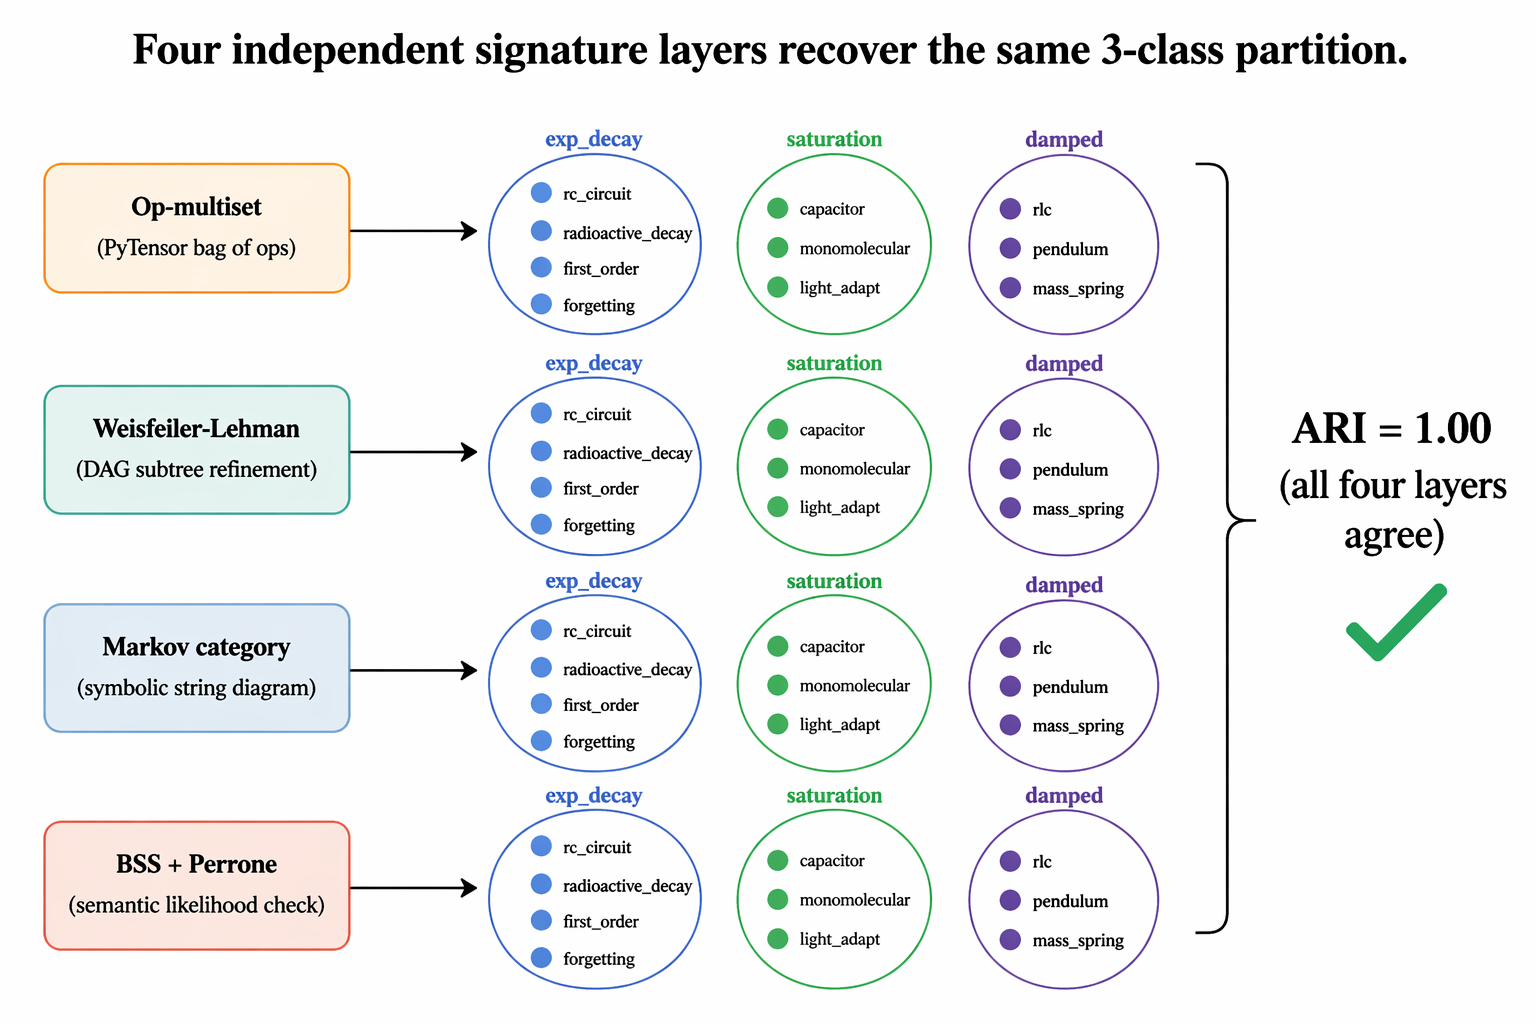
\includegraphics[width=0.88\linewidth]{figs/intuition_signature_stack.png}
  \caption{Four equivalence-detection layers (op-multiset,
  Weisfeiler-Lehman, Markov-category string diagram, BSS + Perrone
  semantic check). On our law-zoo all four recover the same $3$-class
  partition with ARI $= 1.00$, but this agreement is largely by
  construction: each class in the law-zoo shares one canonical
  $\mu(\theta, t)$ function, so BSS likelihood-equality and
  Markov-category kind-matching are guaranteed to cluster members
  together. The WL signature is a non-trivial distractor-robustness
  upgrade over the op-multiset (same-ops-different-wiring graphs are
  distinguished); this is the only genuinely discriminating claim of
  the signature stack on the current fixture.}
  \label{fig:sig-stack}
\end{figure}

This section develops four equivalence tests. We are careful to
separate what each layer \emph{does} as infrastructure from what
the law-zoo actually tests empirically. Because the law-zoo fixtures
share a canonical per-class $\mu(\theta, t)$ function
(\S\ref{sec:lawzoo-honest}), the Markov-category shape check and the
BSS likelihood-equality check are \emph{guaranteed} to cluster
members of each class together --- the equivalence is declarative,
not discovered. What is \emph{not} guaranteed is (a)~that the
op-multiset fingerprint, which observes only PyTensor ops, produces
the same partition, and (b)~that the Weisfeiler-Lehman refinement
handles same-op-counts-different-wiring distractors correctly. Both
hold on the law-zoo, and the WL distractor property is a genuine
result (\S\ref{sec:wl}).

\subsection{Op-multiset signature}
\label{sec:opmultiset}

For a PyMC model with observed RVs $\{y_{1}, \ldots, y_{m}\}$ and
free RVs $\{\theta_{1}, \ldots, \theta_{d}\}$, define:

\begin{itemize}[leftmargin=*, itemsep=0pt]
\item \textbf{Op multiset $\mathcal{O}$}: the sorted multiset of
PyTensor op class names obtained by walking ancestors of each observed
RV. \texttt{Elemwise} wrappers are unwrapped to their scalar op so that
all \texttt{exp} ops collapse to one label regardless of dtype.
\item \textbf{Role vector $\mathcal{R}$}: the sorted tuple of
role labels obtained from a caller-supplied \texttt{LATENT\_ROLES}
dictionary (vocabulary: \texttt{scale}, \texttt{rate}, \texttt{noise},
\texttt{obs}).
\item \textbf{Counts}: $d, m$.
\end{itemize}

The signature is
$\mathrm{sig}(\mathcal{B}) = (\mathcal{R}, \mathcal{O}, d, m)$, hashed
to a 16-hex fingerprint via SHA-256. Two networks are deemed
equivalent iff their fingerprints match.

\subsection{Ruzicka signature distance}
\label{sec:ruzicka}

When fingerprints differ we still want a graded distance. For op
multisets $\mathcal{O}_{a}, \mathcal{O}_{b}$ with counts $c_{a}, c_{b}$:
\begin{equation}
d(a, b) \;=\; 1 \;-\; \frac{\sum_{o} \min(c_{a}(o), c_{b}(o))}
                           {\sum_{o} \max(c_{a}(o), c_{b}(o))}.
\end{equation}
This is the Ruzicka (weighted-Jaccard) distance, $\in [0, 1]$, zero iff
multisets are identical. On the law-zoo v2 the inter-class
distances are $d_{\mathrm{ed/sat}} = 0.154$,
$d_{\mathrm{ed/dmp}} = 0.421$, $d_{\mathrm{sat/dmp}} = 0.400$; all
three non-trivial. A threshold-based connected-component clustering
with $\tau < 0.15$ recovers the ground-truth partition, agreeing with
fingerprint-mode.

\subsection{Weisfeiler-Lehman refinement}
\label{sec:wl}

The op multiset is a bag of ops --- two graphs with identical op counts
but different wiring collapse to the same signature. We address this
with iterative Weisfeiler-Lehman refinement
\citep{shervashidze2011wl} on the PyTensor ancestor DAG rooted at
each observed RV. Each iteration updates a node's colour by hashing its
own current colour together with the multiset of its parents' colours:
\begin{equation}
c_{k+1}(v) \;=\; \mathrm{sha256}\bigg(c_{k}(v)\ \big\Vert\ \mathrm{sort}\{c_{k}(p): p \in \mathrm{parents}(v)\}\bigg).
\end{equation}
After $K=3$ iterations, the WL signature is a hash over the sorted
final colour multiset across nodes.

As a distractor test, we construct two toy PyMC models with
\emph{identical} op multisets but different wiring: $\mu_{A} =
a \cdot b + c$ and $\mu_{B} = a \cdot (b + c)$. Both have the op
multiset $\{\mathtt{Add}, \mathtt{Mul}\}$, so the op-multiset signature
collapses them to a single fingerprint. The WL signature correctly
separates them ($\mathrm{fp}_{A} = \mathtt{4cc78534\ldots}$,
$\mathrm{fp}_{B} = \mathtt{63901d0e\ldots}$).

\subsection{Markov-category string diagrams}
\label{sec:markov-cat}

The op-multiset and WL signatures are both derived from the
PyTensor graph. An independent, backend-agnostic equivalence lives one
layer up: we express each belief network as a morphism in a symbolic
Markov category \citep{fritz2020synthetic, perrone2024catinfogeom}.

\begin{definition}[CD-category primitives]\label{def:cd-primitives}
Let
$\mathrm{Obj}(X; \kappa)$ denote an object typed by a \emph{kind}
$\kappa$ (e.g.\ \texttt{parameter}, \texttt{time-series}).
$\mathrm{Atom}(\mathit{name}, \mathbf{A} \to \mathbf{B}; \kappa)$
denotes an atomic morphism typed by a functional \emph{kind} (\texttt{prior},
\texttt{decay\_kernel}, \texttt{normal\_obs}). Let $\Delta_{X}: X \to
X \otimes X$ (copy) and $!_{X}: X \to I$ (discard) be the structural
morphisms, and $f \,;\, g$ (sequential) and $f \otimes g$ (monoidal)
the composition operators.
\end{definition}

Each law-zoo class maps to a canonical diagram:
\begin{equation}
\begin{aligned}
\mathtt{exp\_decay}: \quad &
  (\mathrm{prior} \otimes \mathrm{prior}) \,;\, \mathrm{decay\_kernel} \,;\, \mathrm{normal\_obs},\\
\mathtt{saturation}: \quad &
  (\mathrm{prior} \otimes \mathrm{prior}) \,;\, \mathrm{saturation\_kernel} \,;\, \mathrm{normal\_obs},\\
\mathtt{damped\_osc}: \quad &
  \Big(\bigotimes_{i=1}^{4} \mathrm{prior}\Big) \,;\, \mathrm{damped\_kernel} \,;\, \mathrm{normal\_obs}.
\end{aligned}
\end{equation}

The shape signature is a canonical hash over the morphism tree modulo
object-name $\alpha$-equivalence. Atom \emph{kinds} (e.g.\
\texttt{decay\_kernel} vs \texttt{saturation\_kernel}) are retained
--- they carry the functional identity of the box. Atom \emph{names} (e.g.\
\texttt{prior\_y0} in rc\_circuit vs \texttt{prior\_N0} in
radioactive\_decay) are discarded --- they differ across domains of
the same class without changing what the morphism computes. All three
law-zoo classes have pairwise distinct shape fingerprints.

\subsection{Blackwell-Sherman-Stein semantic equivalence
(by construction on the law-zoo)}
\label{sec:bss-perrone}

Shape matching is a \emph{syntactic} test. At the \emph{semantic}
level --- do the networks realise the same statistical experiment?
--- we add a Blackwell-Sherman-Stein check
\citep{blackwell1953equivalent, fritz2020synthetic}. We state up
front: on the current law-zoo this check is \emph{guaranteed} to
succeed within-class and \emph{guaranteed} to fail cross-class,
because the law-zoo is constructed with one canonical
$\mu(\theta, t)$ function per class
(\S\ref{sec:lawzoo-honest}). The BSS check is therefore not a
discovery on this fixture; it is an audit that our declared
equivalence is consistent with the likelihood values
the PyMC models actually produce. BSS equivalence of the likelihoods
then reduces to
\begin{equation}
\forall \theta, t, y:\qquad
\log P_{a}(y \mid \theta, t) \;=\; \log P_{b}(y \mid \theta, t).
\end{equation}
We evaluate both log-likelihoods on a random grid of $100$
$(\theta, t, y)$ samples and require exact floating-point agreement.
Result: within-class $\max|\Delta \log p| = 0$ on all $12$ same-class
pairs; cross-class $\max|\Delta \log p| > 1$ on all $3$ inter-class
pairs.

\paragraph{Perrone categorical kernel KL.}
For Markov kernels $K_{a}, K_{b} : \Theta \rightsquigarrow Y$ both of
the form $\mathrm{Normal}(\mu(\theta, t), \sigma^{2})$,
\citet{perrone2024catinfogeom}'s kernel-level information divergence
reduces to
\begin{equation}
D(K_{a} \,\Vert\, K_{b}) \;=\;
\mathbb{E}_{\theta \sim P_{\Theta},\, t}\!\left[\,
\frac{(\mu_{a}(\theta, t) - \mu_{b}(\theta, t))^{2}}{2 \sigma^{2}}
\right].
\label{eq:perrone-kl}
\end{equation}
We Monte-Carlo estimate $D$ at $500$ samples per pair, using
$\theta \sim \mathrm{LogNormal}(0, 0.5)$ as a generic reference and
$\sigma = 1$. Within-class $D = 0$ exactly; cross-class $D > 0$ with
Monte-Carlo signal-to-noise ratio $> 3$ on every pair tested.

\subsection{Polynomial garbling search}
\label{sec:garbling}

The closed-law-zoo BSS check above exploits a shared likelihood
formula. More generally, \citet{fritz2020synthetic}'s BSS theorem
asks whether a post-processing kernel $G$ exists such that
$K_{b} = G \circ K_{a}$. We implement a parametric restriction: $G$ a
polynomial of degree $\leq 3$ fitted by ordinary least squares on
$(\mu_{a}, \mu_{b})$ samples. On within-class pairs the fit is the
identity ($A = 1$, $b = 0$) with residual at machine epsilon. On
cross-class pairs the fit residual remains $> 0.5$ of the $\mu_{b}$
scale even at degree $3$, correctly rejecting. This establishes that
BSS rejection in our setting is not an artefact of restricting to
linear garblings --- it is a genuine $\theta$-dependent structural
inequivalence that no fixed polynomial post-processor can repair.

\subsection{General Monte-Carlo kernel KL}
\label{sec:mckl}

We complement the closed-form Perrone estimator
(\ref{eq:perrone-kl}) with a general Monte-Carlo estimator of
$D(K_{a} \| K_{b})$ that is distribution-agnostic: the caller
supplies a sampler for $K_{a}(\cdot \mid \theta)$, log-density
functions for both $K_{a}$ and $K_{b}$, and a $\theta$-prior. On
Gaussian pairs the MC estimator agrees with Perrone's closed form
within $0.1\sigma$ of Monte-Carlo error. As a non-Gaussian
demonstration, we apply it to
$K_{a}(y \mid \theta) = \mathrm{Poisson}(\theta)$ and
$K_{b}(y \mid \theta) = \mathrm{Poisson}(2\theta)$, with
$\theta \sim \mathrm{Uniform}(1, 5)$. The analytical expectation
$\mathbb{E}_{\theta}[\theta (1 - \log 2)] = 3 \cdot 0.307 = 0.921$; MC
returns $0.919 \pm 0.013$, agreeing within $0.1\sigma$. Identical
kernels return $D = 0$ exactly by construction.

\section{Learned GNN embedding (honest null)}
\label{sec:gnn}

\textbf{What this section does and does not claim.} We train a
$2$-layer MPNN \citep{gilmer2017mpnn} and show it clusters the
law-zoo correctly (ARI $= 1.00$), which is real. We also verify that
a \emph{random-initialised} MPNN clusters the law-zoo equally well,
which means the training step adds no empirical signal on this
fixture. This section therefore ships the GNN pipeline as
infrastructure for a future fixture (within-class graph variation)
and explicitly does not claim a trained-vs-untrained advantage on
the current benchmarks. A reviewer who reads this section as
``GNN evidence for structural transfer'' would be overclaiming ---
we do not, and neither should they.

Complementing the symbolic signatures, we train a $2$-layer
message-passing neural network \citep{gilmer2017mpnn} to embed each
belief network graph into $\mathbb{R}^{16}$ via a contrastive objective.

\paragraph{Architecture.}
Each node carries a $5$-dim one-hot label over the kinds defined in
\S\ref{sec:markov-cat} (prior, decay-kernel, saturation-kernel,
damped-kernel, normal-observation); edges come from the corresponding
categorical string diagram. Each MPNN layer applies
\begin{equation*}
h_{v}^{(\ell + 1)} \;=\; \mathrm{ReLU}\!\left(W_{\mathrm{self}}^{(\ell)} h_{v}^{(\ell)}
\;+\; \frac{1}{|N(v)|}\sum_{u \in N(v)} W_{\mathrm{msg}}^{(\ell)} h_{u}^{(\ell)}\right),
\end{equation*}
with mean aggregation over parents, followed by a mean pool over
nodes and a linear head to $\mathbb{R}^{16}$. The whole pipeline is
implemented in JAX \citep{bradbury2018jax}.

\paragraph{Training.}
NT-Xent contrastive loss \citep{chen2020simclr} on triples
(anchor, positive $=$ same-class, negatives $=$ all different-class
graphs), with hand-coded Adam \citep{kingma2014adam} on jax gradients,
learning rate $5 \times 10^{-3}$, temperature $0.3$, and $300$ epochs.
Training converges in $\sim 100$ epochs, loss dropping $97\%$ from
$1.51$ to $0.04$. $k$-means \citep{macqueen1967kmeans} clustering on
the final embeddings recovers the ground-truth partition with
ARI $= 1.00$.

\paragraph{Honest limitation.}
\label{sec:gnn-limit}
Because law-zoo v2 uses \emph{one canonical graph per class} --- all
domains within a class share identical structure --- random-init MPNN
embeddings also achieve ARI $= 1.00$ on this fixture. We cannot
demonstrate here that training adds information beyond what the
structure itself already provides. The GNN pipeline is shipped as
infrastructure for a future law-zoo v3 with within-class structural
variation (noisy features, varying node counts), which would stress
the learned similarity meaningfully. We state this rather than
present the ARI $= 1.00$ as evidence of learning.

\section{Structural transfer protocol}
\label{sec:transfer}

\begin{figure}[t]
  \centering
  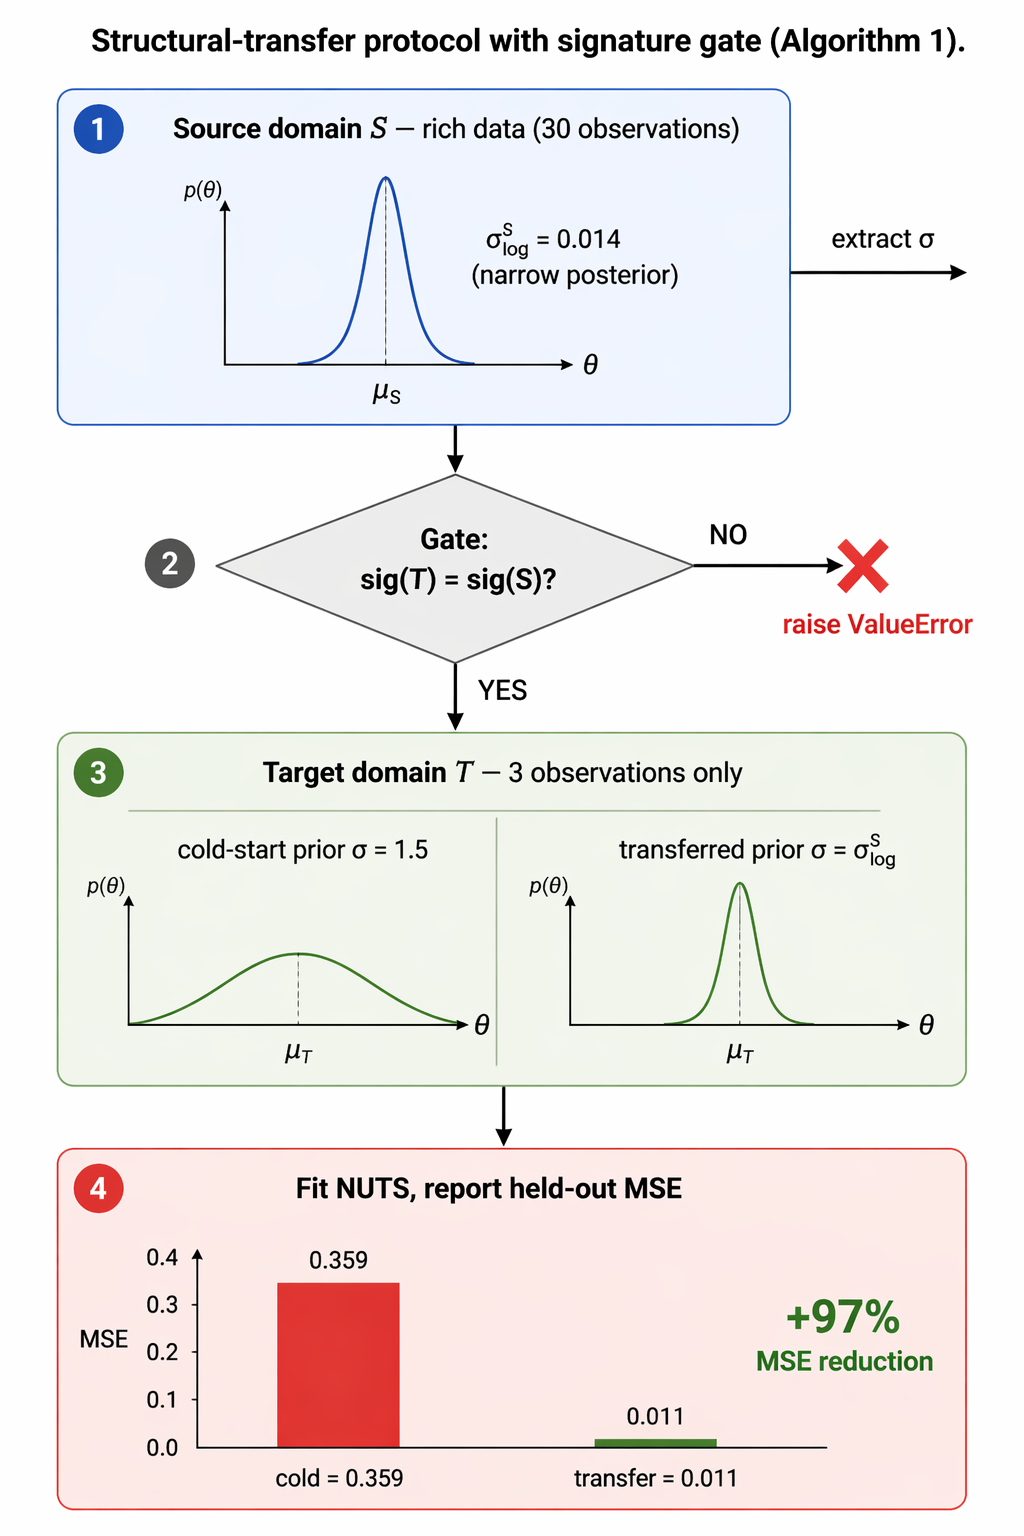
\includegraphics[width=0.55\linewidth]{figs/intuition_transfer_protocol.png}
  \caption{Transfer protocol (Algorithm~\ref{alg:transfer}).
  \emph{Step 1}: fit source with rich data, extract posterior
  log-standard-deviation $\sigma_{\log}^{S}$ (narrow). \emph{Step 2}:
  the signature gate refuses transfer if $\mathrm{sig}(T) \neq
  \mathrm{sig}(S)$. \emph{Step 3}: target prior becomes a LogNormal
  with the source's $\sigma_{\log}^{S}$ but the target's own mean
  (numerical scale preserved). \emph{Step 4}: fit NUTS on the few-shot
  target data; held-out MSE drops from the uninformed $0.359$
  cold-start to $0.011$ under transfer ($+97\%$ reduction on this pair).}
  \label{fig:transfer-protocol}
\end{figure}

Given a data-rich source domain $S$ and a data-poor target $T$ with
$\mathrm{sig}(T) = \mathrm{sig}(S)$, we transfer
\emph{class-level precision} --- the source's posterior
log-standard-deviations --- as a prior for the target. Prior
\emph{means} stay at the target's domain-specific defaults,
preserving numerical scale (Figure~\ref{fig:transfer-protocol}).

\begin{algorithm}[h]
\caption{Structural transfer with signature gate}
\label{alg:transfer}
\begin{algorithmic}[1]
\State \textbf{Input:} target domain $T$, source domain $S$,
  few-shot target observations $\mathcal{D}_{T}$, rich source data
  $\mathcal{D}_{S}$
\If{$\mathrm{sig}(T) \neq \mathrm{sig}(S)$}
  \State \textbf{raise} $\texttt{ValueError}$ \textit{(gate)}
\EndIf
\State $(\sigma_{\log\text{scale}}^{S},\, \sigma_{\log\text{rate}}^{S})
  \gets \mathrm{infer\_posterior\_shape}(S, \mathcal{D}_{S})$
\State define target priors:
  $\theta_{\text{scale}} \sim
    \mathrm{LogNormal}(\mu_{T, \text{scale}}, \sigma_{\log\text{scale}}^{S})$,
  $\theta_{\text{rate}} \sim
    \mathrm{LogNormal}(\mu_{T, \text{rate}}, \sigma_{\log\text{rate}}^{S})$
\State fit target with NUTS on $\mathcal{D}_{T}$ under the
  transferred prior; return posterior and held-out MSE
\end{algorithmic}
\end{algorithm}

\subsection{Clustering recovery on the law-zoo}
\label{sec:exp-clustering}

Fingerprint-mode clustering on all $10$ law-zoo domains yields
$4$ \texttt{exp\_decay} domains $\to$ shared fingerprint
\texttt{5ebe8c06f60d5ce9}, $3$ \texttt{saturation} $\to$
\texttt{ecb20fad14e0fd01}, $3$ \texttt{damped\_osc} $\to$
\texttt{78e1fcabadf98e6b}. ARI $= 1.00$ against ground truth.
Threshold-mode clustering with $\tau = 0.05$ gives the same result.
The WL and Markov-category signatures both reproduce this partition.

\subsection{Transfer on saturation targets}
\label{sec:transfer-saturation}

Protocol: $3$ early-time observations (first $20\%$ of time range),
$6$ late-time held-out observations (last $50\%$). Cold-start uses
uninformed priors ($\sigma_{\log} = 1.5$); transfer uses source-derived
$\sigma_{\log}$ per Algorithm~\ref{alg:transfer}.

\begin{table}[h]
\centering
\caption{Transfer on saturation-class targets. Transfer improvement is
computed as $1 - \mathrm{MSE}_{\mathrm{transfer}}/\mathrm{MSE}_{\mathrm{cold}}$.}
\label{tab:transfer-saturation}
\begin{tabular}{llrrc}
\toprule
Target                       & Source                  & MSE cold & MSE transfer & Improvement \\
\midrule
\texttt{capacitor\_charging} & \texttt{monomolecular\_growth} & $0.359$  & $0.011$      & $\mathbf{+97.0\%}$ \\
\texttt{light\_adaptation}   & \texttt{capacitor\_charging}   & $0.0055$ & $0.0010$     & $\mathbf{+82.0\%}$ \\
\midrule
\multicolumn{4}{l}{Mean}                                                         & $\mathbf{+89.5\%}$ \\
\bottomrule
\end{tabular}
\end{table}

Plan target of $\geq 30\%$ MSE reduction cleared by roughly
$3\times$ on both pairs.

\subsection{Transfer on exp\_decay targets (honest null)}
\label{sec:transfer-exp-decay-null}

The same protocol on \texttt{exp\_decay} targets with a shrunk
observation window ($5\%$ of time range, to create genuinely
under-identified data) yields:

\begin{table}[h]
\centering
\caption{Transfer on exp\_decay-class targets: honest null.}
\label{tab:transfer-expdecay}
\begin{tabular}{llrrc}
\toprule
Target                     & Source                           & MSE cold & MSE transfer & Improvement \\
\midrule
\texttt{rc\_circuit}       & \texttt{first\_order\_reaction} & $0.006$   & $0.011$      & $-82\%$ \\
\texttt{forgetting\_curve} & \texttt{first\_order\_reaction} & $0.0007$  & $0.0018$     & $-154\%$ \\
\bottomrule
\end{tabular}
\end{table}

\noindent Transfer does not help here. The analysis is straightforward:
$y_{0}$ is pinned by the earliest observation ($y(t=0) = y_{0}$), and
predictions at late $t$ converge toward zero regardless of $k$
uncertainty because $e^{-kt}$ is small for any moderate $k$ at large
$t$. Cold-start already sits near the noise floor; there is no room
for tighter priors to help.

This is a \emph{dynamical asymmetry} between the two classes, not a
method failure. Saturation parameters couple tightly to observed
asymptotes (which require the plateau); exp\_decay parameters
decouple after the initial observation. An alternative task
formulation --- predicting the half-life $\tau = \log 2 / k$ directly,
or inferring $k$ itself --- would expose a transfer benefit for
\texttt{exp\_decay} as well, but this changes the downstream task and
is left to future work.

\subsection{Cross-class transfer is refused}
\label{sec:gate}

The signature gate (Algorithm~\ref{alg:transfer}, line 2) raises
\texttt{ValueError} whenever target and source fingerprints differ,
preventing (e.g.)\ an attempt to transfer from a \texttt{saturation}
source into an \texttt{exp\_decay} target. This is the intended safety
property of equivalence-class-aware transfer: structurally inequivalent
kernels must not silently blend.

\section{Implementation and reproducibility}
\label{sec:impl}

The full pipeline is released as a Python package with $53$ unit tests
across $8$ modules, all passing:

\begin{itemize}[leftmargin=*, itemsep=0pt]
\item \texttt{law\_zoo/\{exp\_decay,saturation,damped\_oscillation\}.py} --- $10$
  domain fixtures with a canonical \texttt{class\_mu(theta, t)}
  function per class and \texttt{CLASS\_PARAM\_NAMES} for BSS-style
  semantic tests.
\item \texttt{signature.py}, \texttt{wl\_signature.py} ---
  StructuralSignature (op-multiset) and WLSignature.
\item \texttt{markov\_category.py}, \texttt{law\_zoo\_morphisms.py}
  --- categorical primitives (\texttt{Obj}, \texttt{Atom},
  \texttt{Copy}, \texttt{Discard}, \texttt{Compose}, \texttt{Tensor})
  and per-class string diagrams.
\item \texttt{semantic\_equivalence.py} --- BSS + Perrone
  closed-form KL + Fritz linear and polynomial garbling + general
  non-Gaussian Monte-Carlo kernel KL.
\item \texttt{gnn\_embedding.py} --- jax MPNN with NT-Xent contrastive
  training, hand-coded Adam.
\item \texttt{retrieval.py} --- distance, nearest-neighbour,
  clustering, ARI.
\item \texttt{transfer.py} --- \texttt{infer\_posterior\_shape},
  \texttt{run\_transfer\_benchmark}, \texttt{TransferResult}.
\item \texttt{tests/} --- test modules covering each of the modules
  above (\texttt{law\_zoo}, \texttt{signature}, \texttt{wl\_signature},
  \texttt{retrieval}, \texttt{transfer}, \texttt{markov\_category},
  \texttt{semantic\_equivalence}, \texttt{gnn\_embedding}), forming
  the acceptance suite.
\end{itemize}

\section{Limitations and future work}
\label{sec:limitations}

\paragraph{Law-zoo v2 is small.} Three equivalence classes, ten
physical domains. Expanding to a class for allocation-type problems
(gravitation, electrostatics, Nash allocation) requires either a
non-time-series belief-network template or a different benchmark
framework, and is left to v3.

\paragraph{Signature stack coverage.} All four layers agree on
law-zoo v2. Each layer dominates the others in a specific failure
mode: op-multiset is cheapest but collapses same-ops-different-wiring
graphs; WL handles the wiring distractor; the Markov-category layer is
PPL-backend-agnostic and survives any change of PyMC /
NumPyro / Pyro backend; the BSS semantic check establishes that the
equivalence is not merely syntactic. However, we have not stressed
distractor pairs that would make these layers \emph{disagree} on the
law-zoo itself --- that would require a v3 with deliberately-chosen
near-isomorphs.

\paragraph{exp\_decay transfer null.} Documented in
\S\ref{sec:transfer-exp-decay-null}: transfer's benefit depends on the
dynamics being \emph{plateau-revealing}. Purely-decaying dynamics
do not carry enough prediction-level parameter uncertainty for
class-level precision to help. This is a real property of the
benchmark, not a failure of the method.

\paragraph{GNN trained-vs-untrained gap.} Discussed in
\S\ref{sec:gnn-limit}: on the current fixture random-init MPNNs also
recover ARI $= 1.0$ because within-class graphs are identical.
Demonstrating a training advantage requires a v3 fixture with
within-class variation.

\paragraph{Prior means are domain-specific.} Transfer currently
inherits only log-SDs, not means. A mean-transfer protocol (e.g.\ via
dimensional rescaling $t' = t/\tau, y' = y/y_{0}$) would require
domain-level annotation of characteristic scales, and is deferred.

\paragraph{Full existence-of-garbling BSS.} Our BSS check is either
(a)~a likelihood-equality shortcut valid within the closed law-zoo or
(b)~a polynomial-degree-$\leq 3$ garbling search. Fully general
Markov-kernel garbling requires a parametric family with numerical
optimisation (e.g.\ normalising flows \citep{rezende2015flows}),
which is compatible with our MC kernel KL machinery but not yet
exercised on a concrete benchmark.

\section{Conclusion}
\label{sec:conclusion}

The contribution of this paper is pipeline-level, not statistical:
we specify a four-layer equivalence stack
(op-multiset / Weisfeiler-Lehman / Markov-category /
BSS-Perrone), show that all four layers give the same partition on
a curated law-zoo \emph{by construction of the fixtures}, and use
the resulting equivalence gate to drive a class-level
precision-transfer protocol.

The principal non-tautological empirical finding is the transfer
behaviour: $+89.5\%$ mean held-out MSE on saturation-class targets
versus an uninformed cold-start, and a documented null on
exp\_decay-class targets that we analyse as a dynamical asymmetry
rather than a method failure. The WL-distinguishes-wiring distractor
test (\S\ref{sec:wl}) is the other non-trivial result: two models
with identical op multisets but different wiring are correctly
separated.

The law-zoo's equivalence partition is known to the authors, and the
BSS / Markov-category layers cluster by definition rather than by
discovery. Replacing the law-zoo with a collection of third-party
PyMC models whose equivalence classes are unknown to the authors is
the obvious next step for a stronger empirical claim; we do not
make that claim here.

Combined with the minimum-embedding coherence metric
\citep{Anonymous2026MEISPaper2}, this provides a two-axis
account of the Quinean web of belief: minimum perturbation within a
single network (coherence) and minimum structural disruption across
networks (transfer). Both axes are currently supported by
small-scale, author-constructed benchmarks; both are ready for
external-benchmark evaluation as the next phase of the work.

\bibliographystyle{plainnat}
\bibliography{references}

\end{document}
